\documentclass[aspectratio=169]{beamer}
\mode<presentation>
%\usetheme{Warsaw}
%\usetheme{Goettingen}
\usetheme{Hannover}
%\useoutertheme{default}

%\useoutertheme{infolines}
\useoutertheme{sidebar}
\usecolortheme{dolphin}


\setbeamersize{sidebar width left=0pt} % to remove the sidebar
\beamertemplatenavigationsymbolsempty % To remove the navigation symbols on the bottom right.
\setbeamersize{text margin left=10mm,text margin right=10mm} % Specify margins

\usepackage{amsmath}
\usepackage{amssymb}
\usepackage{listings}
\usepackage{enumerate}
\usepackage{hyperref}
\hypersetup{
    colorlinks=true,
    linkcolor=blue,
    filecolor=magenta,      
    urlcolor=cyan,
}
 
\urlstyle{same}

%some bold math symbosl
\newcommand{\Cov}{\mathrm{Cov}}
\newcommand{\Var}{\mathrm{Var}}
\newcommand{\brho}{\boldsymbol{\rho}}
\newcommand{\bSigma}{\boldsymbol{\Sigma}}
\newcommand{\btheta}{\boldsymbol{\theta}}
\newcommand{\bbeta}{\boldsymbol{\beta}}
\newcommand{\bmu}{\boldsymbol{\mu}}
\newcommand{\bW}{\mathbf{W}}
\newcommand{\one}{\mathbf{1}}
\newcommand{\bH}{\mathbf{H}}
\newcommand{\by}{\mathbf{y}}
\newcommand{\bolde}{\mathbf{e}}
\newcommand{\bx}{\mathbf{x}}

\newcommand{\cpp}[1]{\texttt{#1}}

%--------------------------------------------------
\providecommand{\abs}[1]{\lvert#1\rvert}
\providecommand{\norm}[1]{\lVert#1\rVert}
\providecommand{\Blue}[1]{\textcolor{blue}{#1}}
\providecommand{\Red}[1]{\textcolor{red}{#1}}
\newcommand{\celsius}{\ensuremath{^\circ}C}
\newcommand\thfore{\mathord{\therefore}\,}
%------------------------------------------------------------------

\title{Lecture 25. Recursively Defined  Structures}
%\author{\includegraphics[width=.5\textwidth,height=.5\textheight]{lecture4-fig0.png}}

\date{ }
%------------------------------------------------------------------


\begin{document}

\frame[plain]{\titlepage}




\begin{frame}[plain]{Recursive Definition}

 \begin{itemize}
  \item Recursion is also  useful for many problems that do not involve numbers.
  \item In general, a \Blue{recursive definition} of a given \emph{object}~\footnote{ 
      An object could be a number, a mathematical structure, a function, or almost anything else we want to 
         describe.}
         is made up of two parts:
         \begin{itemize}
          \item[{\bf B.}] {\bf Base step} defines the simplest possible object that doesn't depend on anything else, and
          \item[{\bf R.}] {\bf Recursive  step}
             defines more complicated objects recursively that depend on simpler cases.
         \end{itemize}
        
 \end{itemize}

\end{frame}

\begin{frame}[plain]{}

 \begin{itemize}
  \item  {\bf Example 25.1.} A sequence of symbols written together in some order is called a \Blue{string}.
    \Blue{$\lambda$} represents the \Blue{empty string}, and we do not write $\lambda$ after it has been introduced 
    with another string; for example, {\bf cubs$\lambda =$ cubs}.
    A special kind of string called a \Blue{palindrome}~\footnote{Any word that is the same forward as backward,
      such as {\bf racecar} or {\bf HANNAH}}
    can be defined as follows.
    \begin{itemize}
      \item[{\bf B1.}] \Blue{$\lambda$} is a palindrome. \ {\small (\Red{Why do we need to define this?} Think about forming 'otto')}
      \item[{\bf B2.}] Any symbol \Blue{$\mathrm{a}$} is a palindrome.
      \item[{\bf R.}] If \Blue{$x$} and \Blue{$y$} are palindromes, then \Blue{$yxy$} is a palindrome.
    \end{itemize}
  \item We can build up the palindrome {\bf racecar} from the definition as follows.\pause
    \begin{enumerate}
     \item Since it is a symbol, \Blue{e} is a palindrome by \Blue{B2}. \pause
     \item Similarly, \Blue{c} is a palindrome. \pause
     \item Using \Blue{R}, \Blue{cec} is a palindrome. \pause
     \item By \Blue{B2}, \Blue{a} is a palindrome. \pause
      \item By \Blue{R}, \Blue{aceca} is a palindrome. \pause
      \item By \Blue{B2}, \Blue{r} is a palindrome. \pause
      \item Using \Blue{R}, \Blue{racecar} is a palindrome. 
    \end{enumerate}
     
 \end{itemize}

\end{frame}

\iffalse
\begin{frame}[plain]{}

 \begin{itemize}
  \item  {\bf Remark.} A \Blue{palindromic prime}  is a prime number that is also a palindromic number.   
  Palindromicity depends on the base of the number system and its notational conventions, 
  while primality is independent of such concerns. The first few decimal palindromic primes are:
 \[ 2, 3, 5, 7, 11, 101, 131, 151, 181, 191, 313, 353, 373, 383, 727, 757, 787, 797, 919, 929... \]
 
 \end{itemize}
 
 \vspace{1in}
 

\end{frame}

\fi

\begin{frame}[plain]{ }

 {\bf Practice 25.2.} Define a set (or collection) $X$ of strings in the symbols 0 and 1 as follows.
    \begin{itemize}
      \item[{\bf B.}] 0 and 1 are in $X$.
      \item[{\bf R1.}] If $x$ and $y$ are in $X$, so is $xxyy$.
      \item[{\bf R2.}] If $x$ and $y$ are in $X$, so is $xyx$.
    \end{itemize}
    
    \begin{itemize}
      \item[(a)] Explain why the string $01001011 \in X$ using the definition. Build up the string step by step,
    and justify each step by referring to the appropriate part of the definition.
      \item[(b)] Use the induction method to prove that, if $x$ is in $X$, then $x$ has exactly 
       the same number of $0$s and $1$s.
  \smallskip
      \item[(c)] Find a string in the symbols $0$ and $1$ that has the same number of $0$s and $1$s, but
    is not in $X$. %Answer Example 1100. Note that all strings in X start with 01 or 10.
   %Exam2F15 #2
   \end{itemize}
   
 
\vspace{.5in}

\end{frame}

\begin{frame}[plain]{Python Code for Palindrome Testing}
  \begin{columns}[t] % contents are top vertically aligned
     \begin{column}[T]{5cm} % each column can also be its own environment
       \begin{itemize}
          \item[{\bf B1.}] \Blue{$\lambda$} is a palindrome. 
          \item[{\bf B2.}] Any symbol \Blue{$\mathrm{a}$} is a palindrome.
          \item[{\bf R.}] If \Blue{$x$} and \Blue{$y$} are palindromes, then \Blue{$yxy$} is a palindrome.
       \end{itemize}
     \end{column}
     \begin{column}[T]{8cm} % alternative top-align that's better for graphics        
     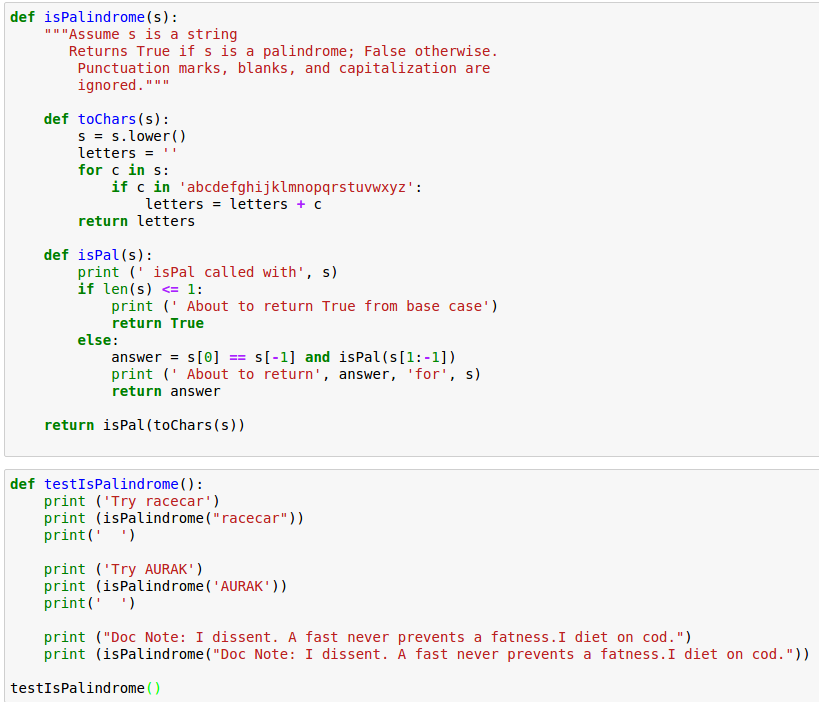
\includegraphics[height=7.3cm]{./img/lecture25-fig1.png}    
     \end{column}
     \end{columns}
\end{frame}

\begin{frame}[plain]{Recursive Geometry}

{\bf Example 25.3}. \Blue{The Koch snowflake fractal}.
     Define a sequence of shapes as follows.
     
     \begin{itemize}
          \item[{\bf B.}] $K(1)$ is an equilateral triangle.
          \item[{\bf R.}] For $n>1, K(n)$ is formed by replacing
             each line segment
      \begin{center}
      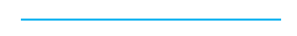
\includegraphics[height=.5cm]{./img/lecture25-fig2a.png}  
     \end{center}
              of $K(n-1)$ with the shape
      \begin{center}
      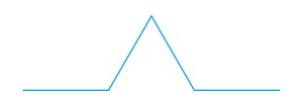
\includegraphics[height=1.6cm]{./img/lecture25-fig2b.png}  
     \end{center}
              
       \end{itemize}
  

   Construct $K(1), K(2)$, $K(3)$, etc.
   \vspace{.5in}
   

\end{frame}

\begin{frame}[plain]{}

  \begin{center}
      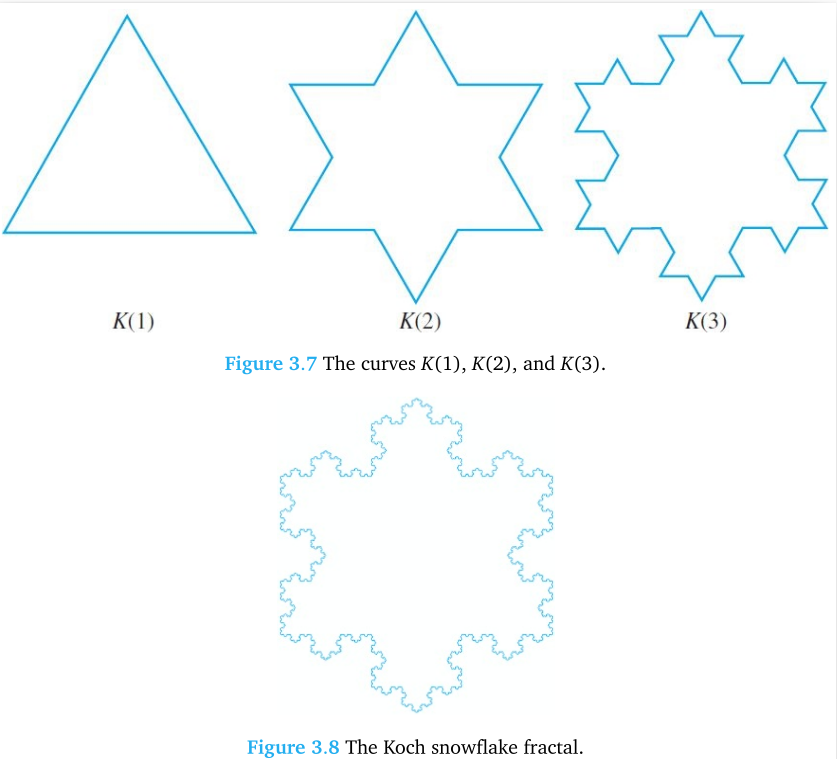
\includegraphics[height=7.5cm]{./img/lecture25-fig2c.png}  
     \end{center}
     
\end{frame}


\end{document}
%%%%%%%%%%%%%%%%%%%%%
 